%% Versión en español del borrador para HardwareX, para revisarlo. El que
%% se envía a la revista es hardwarex.tex (en inglés): si se cambia algo
%% aquí, hay que pasarlo también allá.
%%
%% Todo lo que está en rojo (\TODO{...}) falta. No hay ningún número
%% inventado: los valores salen del código o de mediciones documentadas en
%% el repositorio. Ver LEEME.md.
\documentclass[preprint,12pt]{elsarticle}

\usepackage[T1]{fontenc}
\usepackage[utf8]{inputenc}
\usepackage{lmodern}
\usepackage[spanish,es-noshorthands,es-tabla]{babel}
\usepackage{amsmath}
\usepackage{graphicx}
\usepackage{booktabs}
\usepackage{tabularx}
\usepackage{array}
\usepackage{xcolor}
\usepackage{textcomp}
\usepackage{url}
\expandafter\def\expandafter\UrlBreaks\expandafter{\UrlBreaks\do\_\do\:\do\[}
\Urlmuskip=0mu plus 2mu
\usepackage[hidelinks]{hyperref}

\DeclareRobustCommand{\TODO}[1]{\textcolor{red}{\textbf{[FALTA\ifx\relax#1\relax\else: #1\fi]}}}
\newcommand{\um}{\,\textmu m}
\newcolumntype{L}{>{\raggedright\arraybackslash}X}

\graphicspath{{../capturas/}}

\journal{HardwareX (versión en español para revisión)}
\abstracttitle{Resumen}
\keywordtitle{Palabras clave}

\begin{document}

\begin{frontmatter}

\title{MicroscopeOS: un microscopio abierto de dos cámaras con matriz de
LEDs, integrado a una incubadora, para imagen de células vivas sin marcaje
durante periodos largos, con autoenfoque basado en la fase}

%% FALTA: nombres reales, laboratorio, ciudad y correo.
\author[uanl]{Autor Uno}
\author[uanl]{Autor Dos}
\author[uanl]{Autor de correspondencia\corref{cor1}}
\cortext[cor1]{Autor de correspondencia: nombre@uanl.edu.mx}
\address[uanl]{Laboratorio, Facultad, Universidad Autónoma de Nuevo León,
  Ciudad, Nuevo León, México}

\begin{abstract}
Las células vivas sin teñir son objetos de fase: casi no absorben luz y en
campo claro son prácticamente invisibles, justo en el foco. Los sistemas
comerciales de imagen de células vivas resuelven esto dentro de la
incubadora, pero su costo los deja fuera del alcance de muchos
laboratorios. Presentamos MicroscopeOS, un microscopio de código abierto
construido alrededor de una Raspberry Pi~5 que observa dos muestras
independientes dentro de una cámara con temperatura y CO$_2$ controlados,
en experimentos de timelapse de hasta 48~h. Cada canal óptico tiene su
propia cámara de 8~MP, una matriz programable de $8\times8$ LEDs RGB
controlada por un microcontrolador ESP32-S3 y un eje de enfoque motorizado.
Las matrices de LEDs dan iluminación de campo claro, campo oscuro,
Rheinberg y contraste de fase diferencial (DPC) sin partes móviles. La
misma iluminación de media apertura que se usa para el DPC alimenta un
autoenfoque de dos etapas: el corrimiento lateral, con signo, entre las dos
imágenes de media apertura indica tanto la dirección como la magnitud del
desenfoque, así que el sistema reenfoca sin barridos a ciegas. Las
imágenes DPC se calculan en la Raspberry Pi al terminar cada ciclo, lo que
reduce el almacenamiento de $\sim$65~MB a $\sim$25~MB por cámara y ciclo.
El instrumento se opera desde una interfaz web pensada para usuarios sin
experiencia, accesible en la red local o a distancia a través de un túnel
con autenticación, y envía cada imagen a una estación de trabajo con GPU
para segmentarla en vivo. Todo el software, el firmware y un conjunto de
pruebas que no requiere hardware, con emuladores basados en la física,
están disponibles de forma abierta. \TODO{Una oración con los resultados
principales de la validación (resolución, repetibilidad del autoenfoque,
estabilidad en 48~h, viabilidad celular).}
\end{abstract}

\begin{keyword}
Hardware abierto \sep Imagen de células vivas \sep Contraste de fase
diferencial \sep Microscopía con matriz de LEDs \sep Autoenfoque \sep
Raspberry Pi \sep Timelapse \sep Microscopio de incubadora
\end{keyword}

\end{frontmatter}

%% ---------------------------------------------------------------------------
\section*{Tabla de especificaciones}

\noindent
\begin{tabularx}{\textwidth}{>{\raggedright\arraybackslash}p{0.3\textwidth}L}
\toprule
Nombre del hardware & MicroscopeOS \\
Área & Ciencias biológicas (p.~ej., microbiología y bioquímica);
  herramientas educativas y alternativas abiertas a infraestructura
  existente \\
Tipo de hardware & Herramientas de imagen \\
Equivalente comercial más cercano & Sistemas de imagen de células vivas
  dentro de incubadora, como Sartorius Incucyte o CytoSMART Lux
  \TODO{confirmar y citar el modelo más cercano y su precio} \\
Licencia abierta & \TODO{Elegir y agregar archivos LICENSE al
  repositorio. Sugerencia: GPL-3.0 (software y firmware) y CERN-OHL-S-2.0
  (archivos de diseño de hardware)} \\
Costo del hardware & \TODO{Total de la lista de materiales, en USD} \\
Repositorio de los archivos & \TODO{DOI de Zenodo/OSF/Mendeley Data
  (HardwareX no acepta solo GitHub)}; repositorio de desarrollo:
  \url{https://github.com/AFMMenchacalab/microscopeos-pi5} \\
\bottomrule
\end{tabularx}

%% ---------------------------------------------------------------------------
\section{El hardware en contexto}

La migración celular, dirigida y aleatoria, está detrás del desarrollo
embrionario, la cicatrización y la invasión del cáncer \cite{Ref003}.
Medirla exige observar células vivas durante muchas horas en condiciones
fisiológicas, y después segmentarlas y seguirlas
\cite{WuWirtz2026Methods}. Dos dificultades lo encarecen. Primero, las
células deben mantenerse a 37\,\textdegree C y con CO$_2$ controlado
durante todo el experimento, lo que obliga a meter el microscopio en una
incubadora o a construir una incubadora a su alrededor. Segundo, las
células sin teñir son objetos de fase: retrasan el frente de onda en lugar
de absorberlo, así que en campo claro su contraste es proporcional al
desenfoque y desaparece en el foco. Los marcadores fluorescentes resuelven
el contraste, pero suman fototoxicidad en adquisiciones largas
\cite{Icha2017,Laissue2017}. El contraste de fase clásico
\cite{Zernike1942} y la iluminación asimétrica
\cite{Kachar1985,Mehta2009} recuperan el contraste por vía óptica, y las
matrices de LEDs programables hicieron posibles estas modalidades, incluido
el contraste de fase diferencial (DPC) cuantitativo, por software y sin
óptica especial
\cite{Zheng2011LED,Liu2014LED,Tian2014DPC3D,Tian2015DPC,Lee2015Color,Chen2018DPCaberr}.

Los microscopios comerciales de incubadora integran todo esto, pero a un
precio que limita el acceso, un argumento recurrente a favor de la
instrumentación abierta \cite{Ref027,Ref024,Ref023,Ref026}. Los
microscopios abiertos ya son plataformas maduras: OpenFlexure
\cite{Collins2020OFM}, UC2 \cite{Ref040}, el laboratorio de
\texteuro100 \cite{Ref043}, PlanktoScope \cite{Ref036}, ESPressoscope
\cite{Ref032}, Trackoscope \cite{Ref029} y microscopios abiertos
automatizados de fluorescencia \cite{Ref030}; además, ya se demostró
microscopía computacional con matriz de LEDs y bajo costo sobre hardware
Raspberry Pi \cite{Ref042}. Para imagen de células vivas durante periodos
largos, el Incubot coloca dentro de una incubadora de cultivo un
microscopio basado en una impresora 3D \cite{Merces2021}; otros trabajos
ofrecen control abierto de temperatura o de CO$_2$
\cite{OCarroll2023,Talebipour2024,Rossi2022,Chen2021PrintrLab}, adaptan
OpenFlexure a células vivas \cite{Kearns2026OFMLive} o construyen
plataformas de timelapse impresas en 3D para usarse dentro de la
incubadora \cite{Sato2026DIY}. La reproducibilidad de estos instrumentos
depende de publicar archivos de diseño completos y su validación
\cite{Ref025}.

Hasta donde sabemos, ningún instrumento abierto reúne en un solo equipo:
(i) dos canales ópticos independientes, para observar dos condiciones en
el mismo experimento; (ii) contraste computacional sin marcaje (DPC, campo
oscuro y Rheinberg) con una matriz de LEDs programable por canal; (iii) un
autoenfoque que reutiliza la iluminación del DPC para obtener la
\emph{dirección} del desenfoque, a partir del autoenfoque por iluminación
usado en escaneo de laminillas \cite{Liao2016Autofocus} y no de barridos
de nitidez ni de redes entrenadas \cite{Pinkard2019,Luo2021Autofocus};
(iv) control ambiental registrado con cada imagen; y (v) procesamiento en
el propio equipo, envío de datos y operación remota con autenticación,
para experimentos sin supervisión. \TODO{Comprobar esta afirmación contra
la literatura más reciente antes de enviar.}

%% ---------------------------------------------------------------------------
\section{Descripción del hardware}

MicroscopeOS (Fig.~\ref{fig:arquitectura}) se organiza en cinco subsistemas
que se comunican con una Raspberry Pi~5, la cual se encarga de toda la
adquisición, el procesamiento y el servidor web.

\begin{figure}[ht]
\centering
\fbox{\parbox[c][5cm][c]{0.9\textwidth}{\centering
\TODO{Diagrama de la arquitectura: la Raspberry Pi 5 al centro; CSI hacia
las dos cámaras IMX219; USB serial hacia las dos matrices de LEDs
ESP32-S3; bus UART compartido hacia los dos drivers TMC2209 y los motores
NEMA 11; USB serial hacia el Arduino con DS18B20, SCD30, calefactor y
válvula de CO$_2$; red hacia el navegador, la estación con GPU, el NAS y
el túnel de acceso remoto. La versión en texto está en el README del
repositorio.}}}
\caption{Arquitectura del sistema.}
\label{fig:arquitectura}
\end{figure}

\paragraph{Imagen} Cada canal usa una Raspberry Pi Camera Module~2
(Sony IMX219, $3280\times2464$ píxeles, píxel de 1.12\um) en su propio
puerto CSI de la Raspberry Pi~5, así que las dos cámaras capturan realmente
en paralelo, sin multiplexor. Las imágenes se guardan como TIFF de 16 bits
a la resolución nativa del sensor, a partir de los datos Bayer en crudo.
\TODO{Describir el objetivo (configurado hoy como 20$\times$/NA~0.4 en
\path{core/optica.py}), la lente de tubo o el adaptador y el camino óptico;
dar la escala en \textmu m/píxel medida con un portaobjetos
micrométrico.}

\paragraph{Iluminación programable} Cada canal tiene una placa Waveshare
ESP32-S3-Matrix con una matriz de $8\times8$ LEDs RGB WS2812B debajo de la
muestra. El microcontrolador corre un firmware propio
(\path{codigo/extras/matrices_esp32s3_matrix/}) que recibe comandos de
texto por USB serial (\path{PATRON:brillo[:RRGGBB]}) y confirma cada uno.
Los patrones incluyen apertura completa (campo claro), las cuatro medias
aperturas (izquierda, derecha, arriba, abajo) para el DPC, un anillo
exterior (campo oscuro) y un patrón de dos colores, centro más anillo
(Rheinberg). Cada placa se identifica con una regla udev
(\path{/dev/matriz_cam0}, \path{/dev/matriz_cam1}), sin importar el orden
en que el USB las enumere. \TODO{Distancia de la matriz a la muestra y la
apertura numérica de iluminación resultante.}

\paragraph{Enfoque} Cada canal tiene un motor a pasos NEMA~11
(28HB30-401A, 0.6~A/fase, 1.8\textdegree/paso) sobre una plataforma lineal
con husillo T6$\times$1, así que un paso completo mueve la plataforma
5\um; con el micropaso interno de 1/256 del driver, la resolución nominal
es de $\sim$0.02\um. Los dos motores se manejan con drivers TMC2209 en un
solo bus UART compartido, en modo de varias direcciones, lo que permite al
software cambiar el micropaso y la corriente en caliente y leer el estado
del driver. El juego mecánico se evita llegando siempre a la posición final
desde el mismo sentido. No hay finales de carrera; el software limita a
250\um{} la deriva total del foco permitida durante un timelapse
(\texttt{DERIVA\_MAXIMA\_UM}).

\paragraph{Control ambiental} Un Arduino aparte (Uno/Nano) corre un lazo
PID de temperatura (sensor DS18B20, calefactor por PWM; consigna
37\,\textdegree C, con la salida limitada en rampa para evitar
sobretiro) y un PID proporcional en el tiempo para el CO$_2$ (sensor
Sensirion SCD30, válvula solenoide; consigna 4\%), y reporta la
telemetría en JSON por serial. Tener el lazo de control en su propio
microcontrolador lo hace independiente de los tiempos de la Raspberry Pi
mientras esta escribe archivos TIFF de 16~MB. \TODO{Describir la cámara:
volumen, material, aislamiento, potencia del calefactor, fuente de CO$_2$
y humidificación.}

\paragraph{Cómputo y software} La Raspberry Pi~5 corre MicroscopeOS, una
aplicación en Python (servidor FastAPI, \texttt{picamera2}) que systemd
arranca al encender. Las funciones principales del software son:
\begin{itemize}
\item \textbf{Timelapse} con captura secuencial o simultánea de las dos
  cámaras, telemetría ambiental por ciclo, reenfoque opcional cada $N$
  ciclos y reanudación automática después de un corte de luz (la Pi espera
  a sincronizar la hora por red, porque no tiene pila de reloj, y a que se
  monte el almacenamiento).
\item \textbf{DPC calculado en el equipo} al terminar cada ciclo
  (\path{core/dpc.py}): cada imagen de media apertura se normaliza primero
  por su propio fondo suavizado, porque en nuestro montaje las dos mitades
  de la matriz difieren en brillo hasta el doble; después se calculan
  $\mathrm{DPC} = (I_L - I_R)/(I_L + I_R)$ y la imagen análoga
  arriba--abajo, y se guardan como TIFF de 16 bits comprimidos sin pérdida,
  junto con una suma de campo claro a media resolución. Las cuatro
  imágenes crudas se borran solo después de comprobar que el resultado
  quedó bien escrito en disco. De forma opcional se recupera la fase
  cuantitativa por deconvolución de Tikhonov con las funciones de
  transferencia de objeto débil \cite{Tian2015DPC}.
\item \textbf{Metadatos en cada imagen}: objetivo, tamaño de píxel,
  iluminación, exposición, posición del foco, temperatura y experimento,
  en etiquetas compatibles con ImageJ para que Fiji \cite{Ref079} abra cada
  imagen con su escala física, más una etiqueta JSON con el registro
  completo.
\item \textbf{Conteo de células} en el vivo y en las capturas, con un
  detector clásico (no aprendido) de energía local a la escala de una
  célula y un filtro de calidad que distingue un campo vacío (o la luz
  apagada) de un cultivo confluente; en un timelapse produce una curva de
  población y el tiempo de duplicación.
\item \textbf{Envío de datos}: cada imagen se manda por la red local a una
  estación de trabajo con GPU, que se encuentra sola por difusión UDP y se
  empareja con un código de 6 dígitos, donde se segmenta al llegar con
  Cellpose-SAM \cite{Ref068,Pachitariu2025CellposeSAM}; los envíos se
  verifican con SHA-256 y pasan por una cola, así que un corte de red no
  detiene ni pierde el timelapse. Las imágenes también se pueden respaldar
  en un NAS por SMB o guardar en una memoria USB.
\item \textbf{Interfaz web} (Fig.~\ref{fig:ui}) organizada en cuatro pasos
  numerados (enciende la luz, mira la muestra, enfoca, toma una foto o un
  timelapse), con vivo simultáneo de las dos cámaras, enfoque con el
  teclado, galería de imágenes y exportación con marca de agua y barra de
  escala.
\item \textbf{Acceso remoto}: la Raspberry Pi abre un túnel cifrado de
  salida (Cloudflare Tunnel), así que no se abre ningún puerto de entrada
  en la red de la institución; el acceso se limita a una lista de miembros
  del laboratorio que entran con un código de un solo uso enviado por
  correo (Cloudflare Access).
\end{itemize}

\begin{figure}[ht]
\centering
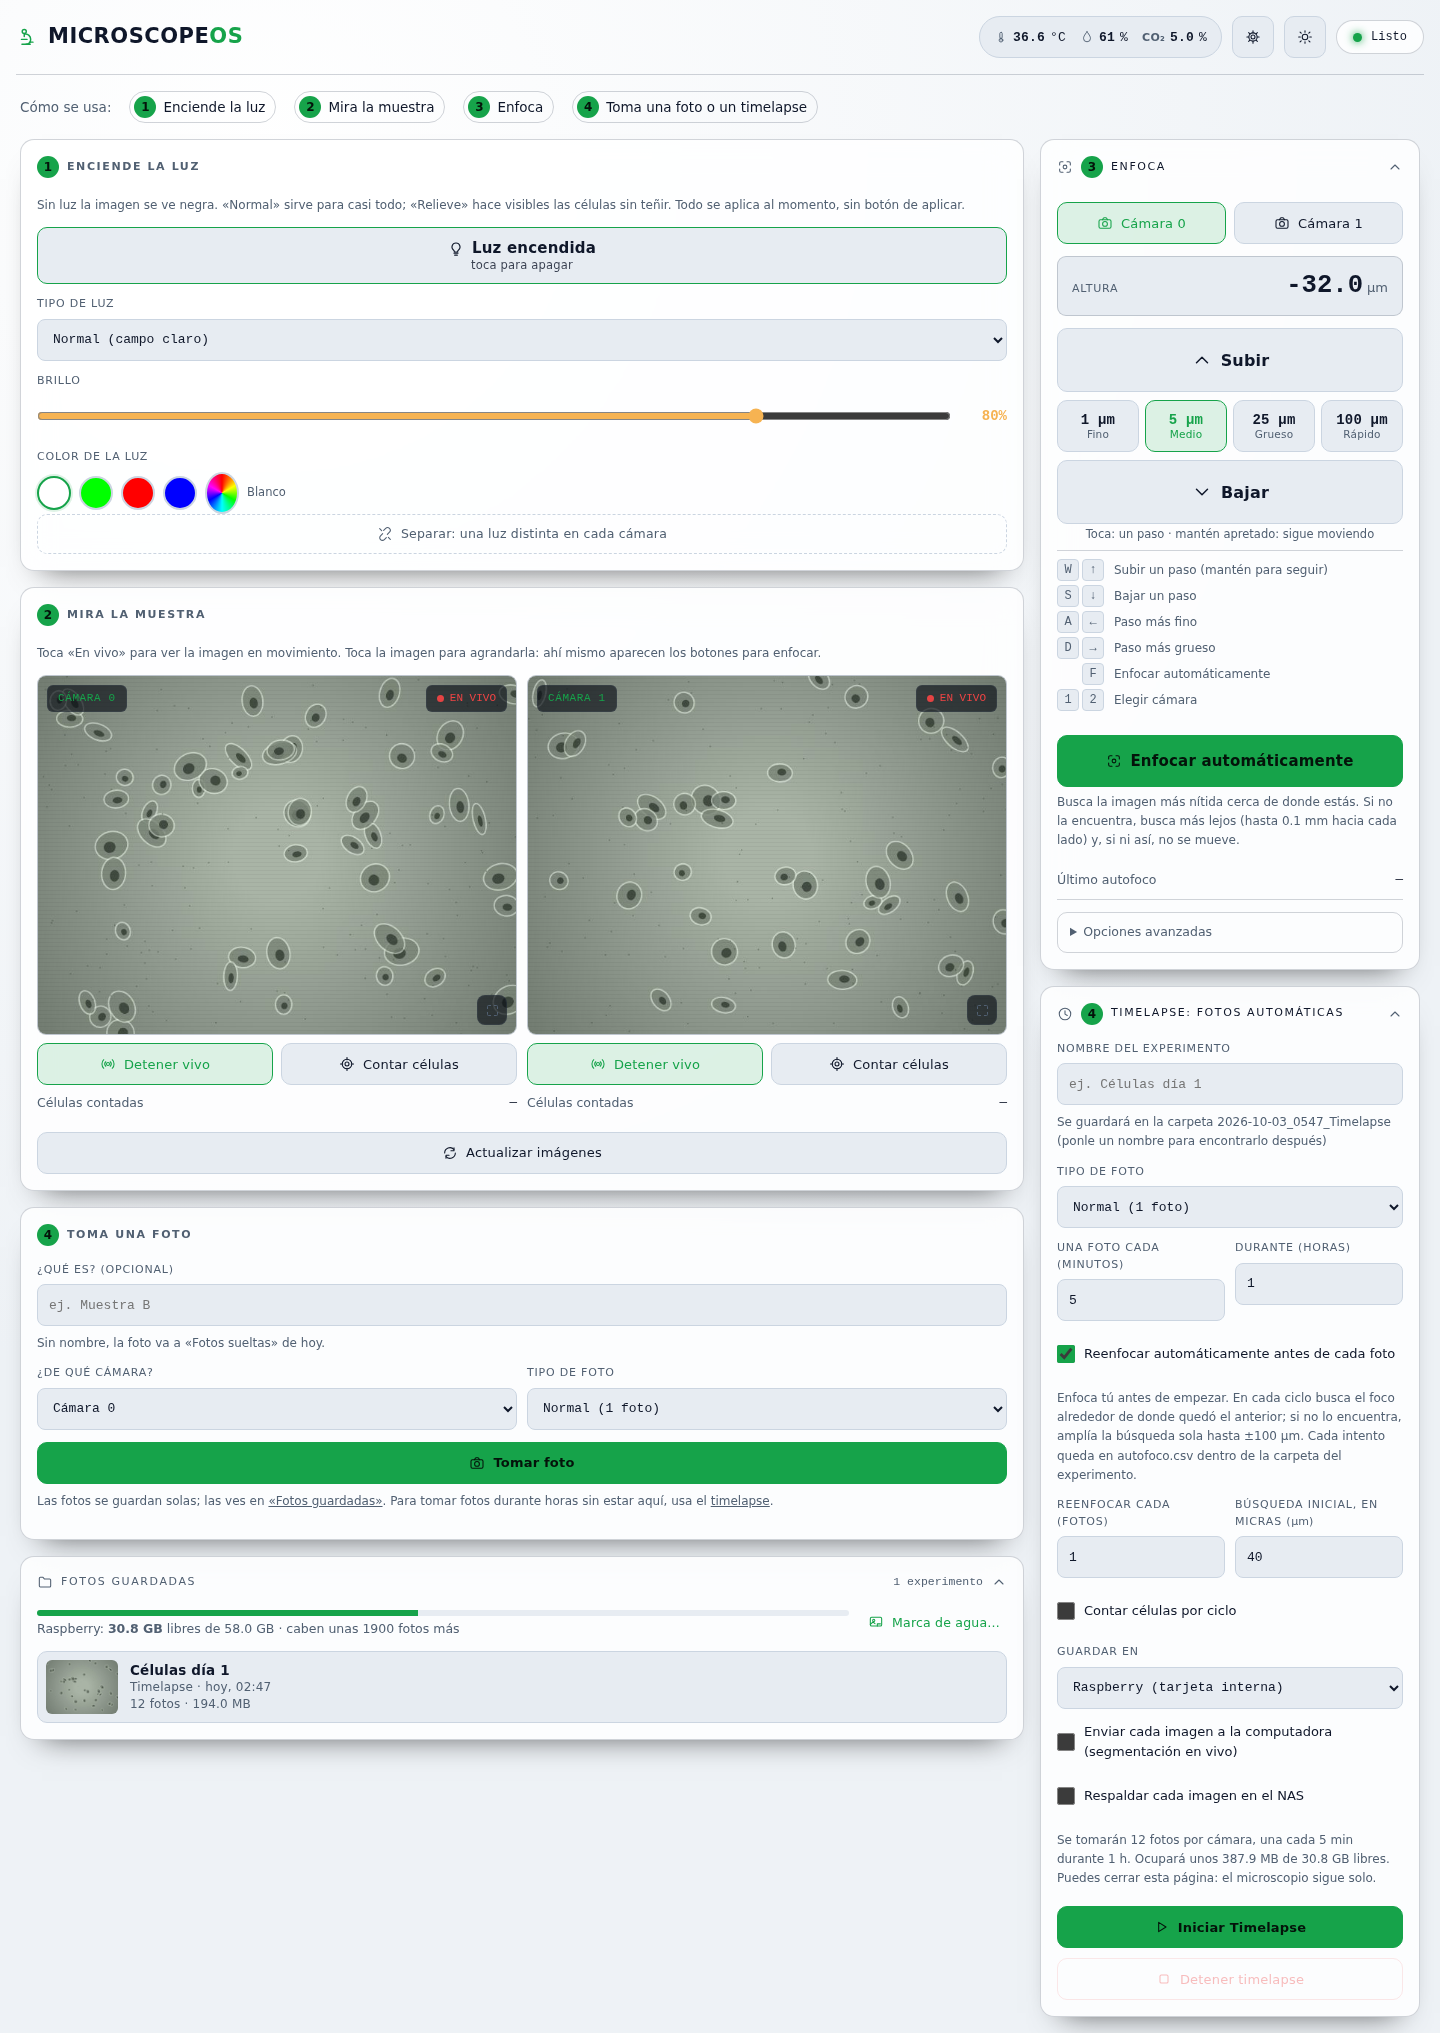
\includegraphics[width=0.9\textwidth,trim=0 1133 0 0,clip]{web_pagina.png}
\caption{Interfaz web. Captura tomada con el microscopio simulado que se
usó para generar el instructivo; la página es la misma que sirve el
instrumento. \TODO{Reemplazar o complementar con una captura del
instrumento real con células reales.}}
\label{fig:ui}
\end{figure}

\paragraph{Autoenfoque} Con iluminación de media apertura, un plano
desenfocado se proyecta de lado, y hacia lados opuestos según qué mitad de
la matriz esté encendida. Por eso el corrimiento lateral entre las imágenes
izquierda y derecha tiene un signo que indica la dirección del desenfoque y,
dentro de un rango lineal, una magnitud proporcional a la distancia al
foco. MicroscopeOS estima el corrimiento por correlación de fase con
precisión de subpíxel y reenfoca en dos etapas. (1) Un salto grueso con
dirección: después de una calibración única por objetivo (un barrido de
$\pm$12\um{} que ajusta la recta corrimiento contra posición), una sola
medición da la distancia al cruce por cero y la plataforma va directo
ahí. (2) Ajuste fino: como cerca del foco una sola lectura es ruidosa, el
corrimiento se mide en 7 planos cercanos y se toma la mediana de las 7
estimaciones del cruce por cero. Si el sistema no está calibrado, si la
correlación es débil (campo vacío) o si una corrección aleja del foco, la
plataforma vuelve al inicio y un barrido de grueso a fino busca el mismo
criterio (el cruce por cero del corrimiento), así que los dos métodos
terminan en el mismo plano. La búsqueda empieza en $\pm$20\um{} y se
amplía hasta $\pm$100\um{} si hace falta. Evitamos a propósito las
métricas de nitidez: la métrica de Tenengrad calculada sobre imágenes DPC
es casi plana cerca del foco con células sin teñir y tiene un
\emph{mínimo} local en el foco con muestras que absorben, lo que hacía que
el autoenfoque por nitidez terminara en un plano distinto cada vez. El
barrido de calibración ($\pm$12\um) se eligió para quedar dentro del rango
en que el corrimiento es lineal ($\sim\pm$15\um{} en nuestro montaje).

\paragraph{Cómo ayuda este hardware a los investigadores}
\begin{itemize}
\item Observa dos muestras o condiciones en paralelo, cada una con su
  propio enfoque e iluminación, hasta 48~h con temperatura y CO$_2$
  controlados.
\item Da contraste sin marcaje de células sin teñir (DPC) sin objetivos de
  contraste de fase, evitando la fototoxicidad de la fluorescencia.
\item Reenfoca solo durante experimentos largos, con la misma iluminación
  del modo de contraste.
\item Cada imagen lleva su escala física y sus condiciones de adquisición,
  y el equipo reduce el almacenamiento sobre la marcha al calcular el DPC.
\item Se opera desde cualquier navegador, por usuarios sin capacitación
  previa, en el laboratorio o a distancia, y envía las imágenes a una
  estación de trabajo para analizarlas en vivo.
\item Todo el software se puede probar sin hardware, con emuladores de la
  cámara (incluida la física del DPC), de las matrices de LEDs y de los
  drivers de los motores.
\end{itemize}

%% ---------------------------------------------------------------------------
\section{Resumen de los archivos de diseño}

\noindent
\begin{tabularx}{\textwidth}{>{\raggedright\arraybackslash}p{0.33\textwidth}
  >{\raggedright\arraybackslash}p{0.14\textwidth}
  >{\raggedright\arraybackslash}p{0.17\textwidth}L}
\toprule
Archivo de diseño & Tipo & Licencia abierta & Ubicación \\
\midrule
MicroscopeOS (adquisición, procesamiento, servidor web) & Python, HTML &
  \TODO{} & \path{codigo/MicroscopeOS/} \\
Firmware de las matrices de LEDs (\path{dpc_matrix.ino}) & Arduino (C++)
  & \TODO{} & \path{codigo/extras/matrices_esp32s3_matrix/} \\
Firmware del PID de la incubadora
  (\path{Control_Incubator_TempCO2.ino}) & Arduino (C++) & \TODO{} &
  \path{codigo/extras/incubadora_temperatura/} \\
Entrenamiento del autoenfoque aprendido (opcional) & Python & \TODO{} &
  \path{codigo/extras/ia/} \\
Configuración del sistema (arranque, udev, systemd, ejemplo del túnel) &
  Texto & \TODO{} & \path{configs/} \\
Pruebas sin hardware y emuladores & Python & \TODO{} & \path{tests/} \\
Instructivo de uso & PDF, HTML & \TODO{} & \path{docs/instructivo/} \\
\TODO{Piezas mecánicas (soportes de cámara, portamuestras, soporte de la
  matriz, piezas de la platina de enfoque)} & \TODO{STL + STEP} & \TODO{}
  & \TODO{todavía no están en el repositorio} \\
\TODO{Diseño de la cámara de incubación y diagrama de cableado} &
  \TODO{PDF/SVG} & \TODO{} & \TODO{todavía no están en el repositorio} \\
\bottomrule
\end{tabularx}

\medskip\noindent
\TODO{Una oración que describa cada archivo de diseño, como pide la
revista.}

%% ---------------------------------------------------------------------------
\section{Resumen de la lista de materiales}

\noindent\TODO{Llenar costos unitarios y proveedores (marcados con ?) y
números de parte. Los componentes son los del instrumento tal como está
armado.}
\medskip

\noindent
\begin{tabularx}{\textwidth}{>{\raggedright\arraybackslash}p{0.38\textwidth}
  >{\centering\arraybackslash}p{0.07\textwidth}
  >{\centering\arraybackslash}p{0.12\textwidth}
  >{\centering\arraybackslash}p{0.12\textwidth}L}
\toprule
Componente & Cant. & Costo unitario (USD) & Total (USD) & Proveedor \\
\midrule
Raspberry Pi 5 (8 GB) & 1 & ? & ? & ? \\
Fuente de la Raspberry Pi 5 (27 W) & 1 & ? & ? & ? \\
Tarjeta microSD / almacenamiento & 1 & ? & ? & ? \\
Raspberry Pi Camera Module 2 (IMX219) & 2 & ? & ? & ? \\
Cables CSI para Raspberry Pi 5 & 2 & ? & ? & ? \\
Objetivo de microscopio \TODO{modelo} & 2 & ? & ? & ? \\
Waveshare ESP32-S3-Matrix ($8\times8$ WS2812B) & 2 & ? & ? & ? \\
Motor a pasos NEMA 11 28HB30-401A & 2 & ? & ? & ? \\
Plataforma lineal con husillo T6$\times$1 (28T0601-50) & 2 & ? & ? & ? \\
Driver de motor a pasos TMC2209 & 2 & ? & ? & ? \\
Fuente para los motores \TODO{voltaje} & 1 & ? & ? & ? \\
Arduino Uno/Nano & 1 & ? & ? & ? \\
Sensor de temperatura DS18B20 & 1 & ? & ? & ? \\
Sensor de CO$_2$ Sensirion SCD30 & 1 & ? & ? & ? \\
Calefactor \TODO{tipo, potencia} y driver MOSFET & 1 & ? & ? & ? \\
Válvula solenoide de CO$_2$ y regulador & 1 & ? & ? & ? \\
Cámara, piezas impresas en 3D, tornillería & -- & ? & ? & ? \\
\midrule
\textbf{Total} & & & ? & \\
\bottomrule
\end{tabularx}

%% ---------------------------------------------------------------------------
\section{Instrucciones de armado}

\TODO{Armado mecánico paso a paso, con fotos: estructura, platinas de
enfoque, soportes de cámara y objetivo, soportes de las matrices, cámara
de incubación, calefactor, sensores y línea de CO$_2$. HardwareX pide
suficiente detalle para que alguien más pueda reproducir el instrumento,
con advertencias de seguridad.}

\paragraph{Electrónica} \TODO{Diagrama de cableado.} Los dos drivers
TMC2209 comparten una línea UART conectada a los GPIO14/15 de la Raspberry
Pi, cada uno configurado con una dirección distinta; la asignación completa
de pines está documentada en \path{core/motor_focus.py}. Las matrices de
LEDs y el Arduino se conectan por USB.

\paragraph{Instalación del software} En Raspberry Pi OS (64 bits), los
paquetes que dependen del hardware (\texttt{picamera2}, OpenCV, NumPy,
pyserial, GPIO) se instalan con \texttt{apt}, y el resto de las
dependencias en un entorno virtual que hereda los paquetes del sistema. La
configuración de arranque habilita las dos cámaras IMX219 y el UART de los
drivers, las reglas udev dan nombres fijos a las matrices de LEDs y una
unidad de systemd arranca el servidor al encender. El firmware de las
matrices y del controlador de la incubadora se carga con las herramientas
de Arduino, usando las versiones de las bibliotecas fijadas en el
repositorio. El acceso remoto se configura con \texttt{cloudflared}; se
incluye un ejemplo de configuración sin credenciales. Los comandos
completos están en el README del repositorio.

%% ---------------------------------------------------------------------------
\section{Instrucciones de operación}

El instrumento se opera desde un navegador web en la dirección de la
Raspberry Pi. La interfaz guía al usuario en cuatro pasos: (1) encender la
luz y elegir la iluminación (normal, de campo claro, o ``relieve'' (DPC)
para células sin teñir), el brillo y el color; (2) iniciar el vivo de cada
cámara; (3) enfocar con botones, con el teclado o con el botón de
autoenfoque; (4) tomar una sola imagen o configurar un timelapse (nombre,
modo de iluminación, intervalo, duración, reenfoque, conteo de células,
destino de almacenamiento y envío opcional a la estación de trabajo y al
NAS). Antes de empezar, la interfaz estima el número de imágenes y el
espacio en disco, y el timelapse sigue aunque se cierre el navegador. En
el repositorio se incluye un instructivo impreso de doce páginas para
usuarios sin experiencia, con una tabla de problemas y una tarjeta de
referencia rápida.

\paragraph{Seguridad}
\begin{itemize}
\item Los ejes de enfoque no tienen finales de carrera; un movimiento
  excesivo puede llevar el objetivo contra la muestra. Acercar la muestra a
  mano antes de usar el autoenfoque. \TODO{Agregar topes mecánicos o
  describir el montaje seguro.}
\item Las matrices de LEDs se alimentan por USB; el brillo está limitado
  por software para mantener la corriente dentro del límite del USB.
\item \TODO{Seguridad del calefactor y del tanque de CO$_2$: protección
  contra sobretemperatura, regulación de presión y ventilación.}
\end{itemize}

%% ---------------------------------------------------------------------------
\section{Validación y caracterización}

\paragraph{Validado hasta ahora} En el instrumento armado, las dos cámaras
capturan en paralelo imágenes TIFF de 16 bits a resolución nativa; los
cuatro modos de iluminación responden y se confirmaron visualmente; los
dos ejes de enfoque se mueven correctamente a través del bus UART
compartido; y se verificó que el acceso remoto por el túnel redirige al
inicio de sesión toda petición sin autenticar, incluidos los comandos de
movimiento. El DPC calculado en el equipo se midió con una captura real
de la cámara~0 ($3280\times2464$): cada imagen DPC ocupa 10.6~MB y la suma
de campo claro a media resolución 2.8~MB, es decir $\sim$25~MB por ciclo y
cámara contra $\sim$65~MB de las cuatro imágenes crudas. El ruido por
píxel de la imagen DPC, medido en zonas vacías de la misma muestra, fue de
$\sim$0.008, lo que llevó a guardar el DPC con un paso de 1/4096 (la
cuantización suma alrededor del 1\% de ese ruido).

\paragraph{Pruebas del software} Las pruebas corren sin ningún hardware:
reemplazan la cámara, las matrices de LEDs y los drivers de los motores por
emuladores que hablan los protocolos reales, incluido un modelo de cámara
con la física del DPC (desenfoque, corrimiento con signo bajo media
apertura y objetos de fase cuyo contraste en campo claro desaparece en el
foco). En estas simulaciones, un barrido de nitidez sobre imágenes crudas
de campo claro converge a un plano lejos del foco, mientras que el
criterio del corrimiento DPC converge al foco. En campos sintéticos de 40
células de fase en foco, el contador encuentra 0 células con campo claro y
40 con media apertura o DPC; por eso el conteo en vivo pone la matriz en
media apertura. Estos resultados son de simulación y hay que confirmarlos
con muestras reales.

\paragraph{Caracterización pendiente}
\TODO{Cada punto necesita un experimento y una figura. No se reporta
ningún valor hasta medirlo.}
\begin{enumerate}
\item \textbf{Resolución y campo de visión}: carta USAF 1951 con cada modo
  de iluminación; portaobjetos micrométrico para la escala en
  \textmu m/píxel de cada canal. \TODO{figura + tabla}
\item \textbf{Contraste DPC}: el mismo campo de células sin teñir en campo
  claro, media apertura y DPC; de forma opcional, una referencia de fase
  (microesferas de tamaño e índice de refracción conocidos).
  \TODO{figura}
\item \textbf{Autoenfoque}: exactitud y repetibilidad contra un foco de
  referencia (p.~ej., $n$ repeticiones desde desenfoques conocidos de
  $\pm$10, 25 y 50\um), tiempo por enfoque, rango lineal de la calibración
  y tasa de fallos con campo vacío y con cultivo confluente.
  \TODO{figura + tabla}
\item \textbf{Mecánica}: exactitud del paso de enfoque y juego del husillo,
  medidos con un comparador de carátula o por registro de imágenes.
  \TODO{tabla}
\item \textbf{Estabilidad ambiental en 48~h}: registros de temperatura y
  CO$_2$ (media, desviación estándar, sobretiro) y deriva del foco con y
  sin autoenfoque. \TODO{figura}
\item \textbf{Estabilidad de la iluminación}: intensidad media de la imagen
  durante 48~h. \TODO{figura}
\item \textbf{Viabilidad celular dentro del instrumento}: proliferación o
  viabilidad de \TODO{línea celular, p.~ej., MDA-MB-231} cultivada 48~h en
  el instrumento con el protocolo de imagen, contra un control en una
  incubadora normal. \TODO{figura + estadística}
\item \textbf{Diafonía entre los dos canales}: imágenes con una sola
  matriz encendida. \TODO{figura}
\item \textbf{Ejemplo de aplicación}: un timelapse DPC de 48~h de
  \TODO{línea celular} con segmentación en la estación de trabajo, que
  muestre que los datos sirven para análisis de migración
  \cite{WuWirtz2026Methods}. \TODO{figura}
\end{enumerate}

\paragraph{Limitaciones} La matriz de $8\times8$ limita los patrones de
iluminación y el muestreo angular disponible para la fase cuantitativa; la
fase recuperada depende de la regularización y no tiene corrección de
fondo, así que sus valores absolutos en radianes todavía no son
confiables. Los ejes de enfoque no tienen finales de carrera. El
autoenfoque aprendido opcional está implementado pero no entrenado. El
instrumento todavía no se ha caracterizado de forma cuantitativa (ver
arriba).

%% ---------------------------------------------------------------------------
\section*{Declaraciones éticas}

\TODO{Si solo se usan líneas celulares comerciales: ``Este trabajo no
involucró sujetos humanos ni experimentos con animales.'' Indicar el
origen y la autenticación de las líneas celulares.}

\section*{Contribución de los autores (CRediT)}

\TODO{Roles de cada autor (conceptualización, software, hardware,
validación, redacción del borrador original, \ldots).}

\section*{Declaración de uso de IA generativa}

\TODO{Elsevier pide declarar el uso de IA generativa en la redacción y,
cuando aplique, en el desarrollo del software. Describir las herramientas
usadas y para qué.}

\section*{Declaración de conflicto de intereses}

Los autores declaran que no tienen intereses financieros en competencia ni
relaciones personales conocidas que pudieran haber influido en el trabajo
presentado en este artículo.

\section*{Agradecimientos}

\TODO{Financiamiento y agradecimientos.}

\bibliographystyle{elsarticle-num}
\bibliography{referencias}

\end{document}
